%==============================================================================
% DROP-IN SECTIONS — Interrupted Time-Series analysis
%
% Written against the structure of LLM_AI_Impact.pdf. Each block says where it
% goes. Packages assumed: booktabs, graphicx, amsmath. Nothing exotic.
%
% WHAT THIS CHANGES IN YOUR DOCUMENT
%   §2  add 2.5 (new subsection below)
%   §3.1, §3.2  add the ITS paragraph + Table ITS after the existing tables;
%               Finding 1 and Finding 2 need rewording (replacements below)
%   §5.2  "Absolute Quality Measures" is now largely RESOLVED — replacement below
%   Abstract, §6  replacement paragraphs below
%==============================================================================


%==============================================================================
% [1] NEW SUBSECTION — goes at the end of §2 Methods
%==============================================================================
\subsection{Interrupted Time-Series Specification}
\label{sec:its}

A pre/post comparison cannot separate an intervention effect from a trend that
was already running. A codebase accumulates lines, complexity and rule
violations month after month whether or not an AI tool is present, so an
observation that size is 11\% higher after adoption is consistent both with an
effect of adoption and with the simple passage of time. To distinguish them we
fit an interrupted time series (segmented regression) that estimates the
pre-adoption trend explicitly and asks what occurs on top of it.

For repository $i$ in event month $\tau$, where $\tau = 0$ is that
repository's own adoption month,
\begin{equation}
  y_{i\tau} \;=\; \alpha_i \;+\; \beta_1 \tau \;+\; \beta_2 \mathrm{POST}_{i\tau}
            \;+\; \beta_3 \bigl(\tau \cdot \mathrm{POST}_{i\tau}\bigr)
            \;+\; \varepsilon_{i\tau},
  \label{eq:its}
\end{equation}
with $\mathrm{POST}_{i\tau} = \mathbf{1}[\tau \ge 0]$. The coefficients carry
the following interpretation:

\begin{itemize}
  \item $\alpha_i$ — repository fixed effect. Each repository is compared only
    against itself, so differences in scale between repositories cannot drive
    the estimate.
  \item $\beta_1$ — the \textbf{pre-adoption trend}. This is the
    counterfactual: the rate at which the outcome was already changing.
  \item $\beta_2$ — the \textbf{level change} at adoption, net of $\beta_1$.
  \item $\beta_3$ — the \textbf{slope change} after adoption. A positive
    $\beta_3$ means growth accelerated beyond its prior rate.
\end{itemize}

Outcomes that are strictly positive and vary in scale are logged, so
coefficients read as approximate proportional change and the fixed effects
absorb repository size multiplicatively. Standard errors are clustered by
repository: consecutive months within a repository are strongly
autocorrelated, and treating them as independent would overstate precision.
The window is $\tau \in [-10, +3]$, and a repository enters the estimation
only if it contributes at least three pre-adoption and one post-adoption
month, so that $\beta_2$ and $\beta_3$ are identified from repositories that
actually straddle the event.

\paragraph{Branch scope.} MOSIP follows gitflow, in which \texttt{master} is a
release branch that receives merge commits rather than development. Across the
twenty repositories \texttt{master} holds only a small minority of commits in
the window --- \texttt{registration-client}, for instance, records 2 commits on
\texttt{master} against 39 on \texttt{develop} --- so analysing the nominal
default branch would discard most development activity. We therefore report
velocity on \texttt{origin/develop}, the integration branch, which is also the
branch the SonarQube snapshots follow. This makes the velocity and quality
series describe the same tree for the first time. Results for the
all-branches scope are reported alongside and do not differ for any quality
outcome.


%==============================================================================
% [2] RESULTS — insert after the existing §3.1 and §3.2 tables
%==============================================================================

\begin{table}[htbp]
\centering
\caption{Interrupted time-series estimates. Log outcomes, so $\beta_1$ and
$\beta_3$ read as \% per month and $\beta_2$ as a \% level shift. Repository
fixed effects; standard errors clustered by repository.
\textsuperscript{*}$p<.05$, \textsuperscript{**}$p<.01$,
\textsuperscript{***}$p<.001$.}
\label{tab:its}
\small
\begin{tabular}{@{}lrrrrr@{}}
\toprule
 & $\beta_1$ pre-trend & $\beta_2$ level & $\beta_3$ slope chg. & obs. & repos \\
Outcome & (\%/month) & (\%) & (\%/month) & & \\
\midrule
Code size (ncloc)      & $+1.28$\textsuperscript{***} & $-2.20$\textsuperscript{*}  & $+0.12$ & 181 & 17 \\
Cognitive complexity   & $+1.46$\textsuperscript{**}  & $-2.58$                     & $+0.29$ & 181 & 17 \\
Code smells            & $+1.53$\textsuperscript{**}  & $-3.58$\textsuperscript{**} & $-0.16$ & 181 & 17 \\
Technical debt         & $+0.82$                      & $-4.04$\textsuperscript{*}  & $+0.49$ & 181 & 17 \\
\addlinespace
Commits / month        & $-8.06$\textsuperscript{*}   & $+27.62$                    & $+9.08$ & 181 & 17 \\
Lines added / month    & $-9.66$                      & $+255.4$\textsuperscript{*} & $+1.67$ & 170 & 16 \\
PRs opened / month     & $-4.14$\textsuperscript{*}   & $-17.58$                    & $+17.12$ & 212 & 19 \\
\bottomrule
\end{tabular}
\end{table}

\begin{figure}[htbp]
  \centering
  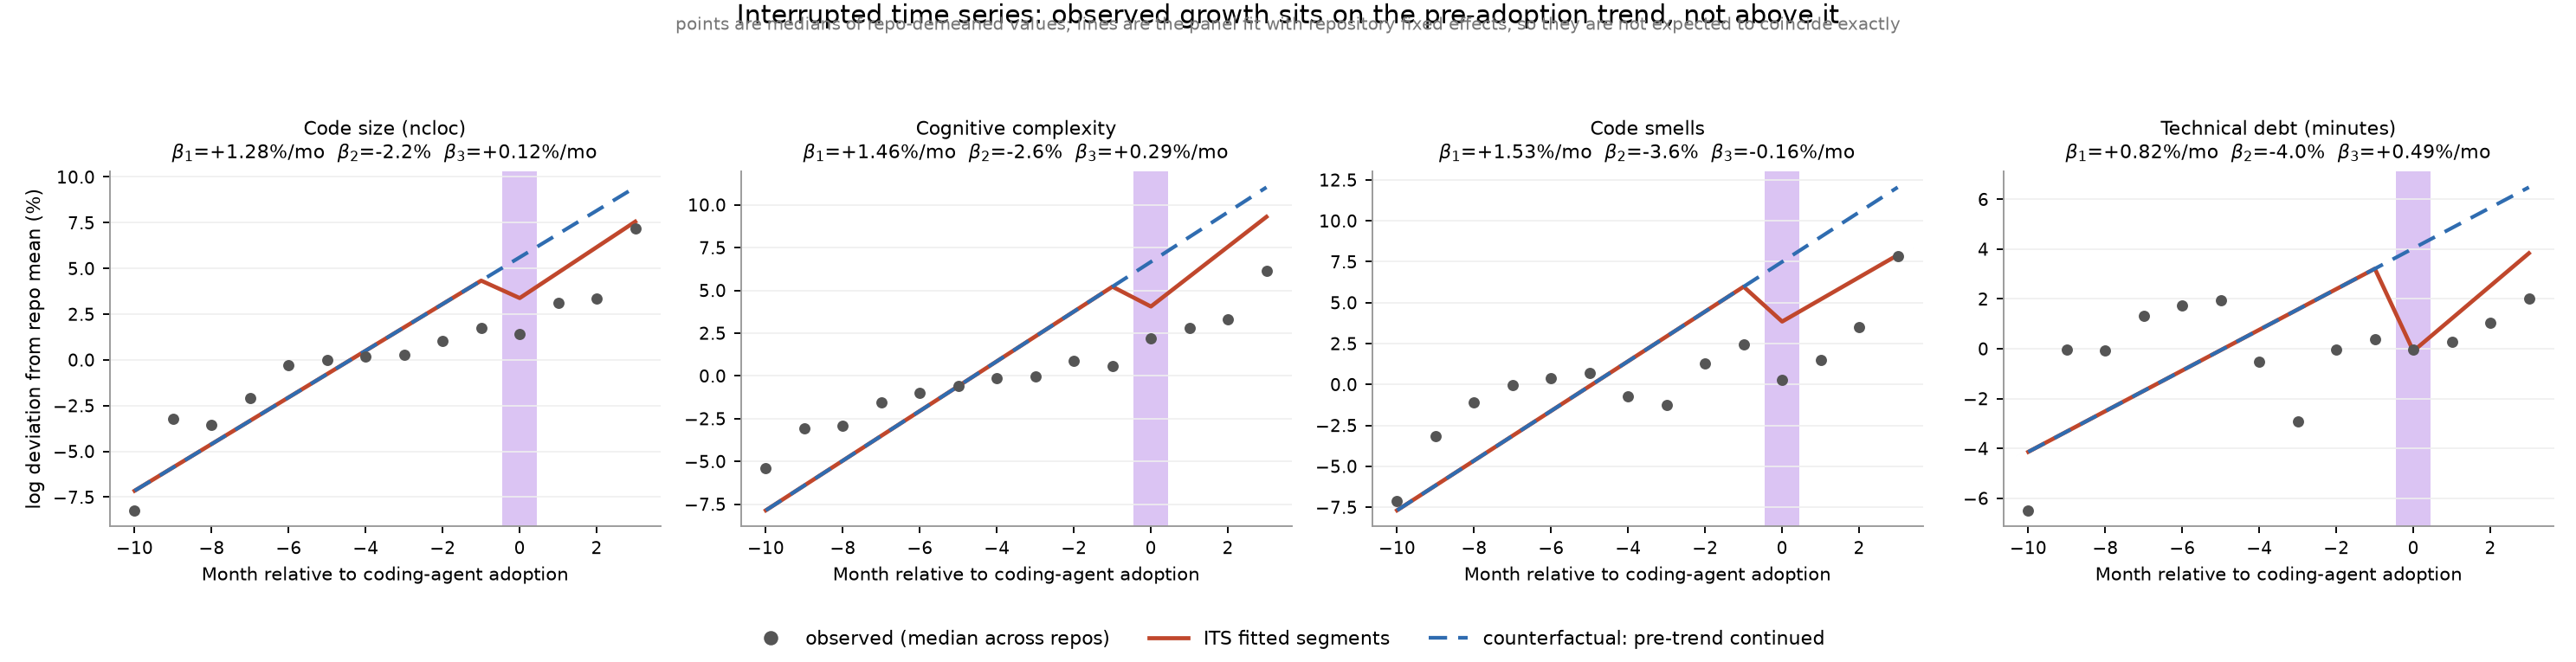
\includegraphics[width=\linewidth]{figures/its.png}
  \caption{Interrupted time series for the four quality and size outcomes.
  Grey points are observed values, taken as the median across repositories
  after removing each repository's own mean. The solid line is the fitted
  segmented regression; the dashed line extends the pre-adoption trend
  ($\beta_1$) past the adoption month and is therefore the counterfactual
  --- what the outcome would have reached had the prior trajectory simply
  continued. In every panel the observed series after adoption lies on or
  below that counterfactual, which is the central result of
  Section~\ref{sec:its-results}: the growth visible in the raw pre/post
  comparison is the continuation of a trend that predates AI adoption.
  Points and lines are not expected to coincide exactly, because the points
  are repository-demeaned medians while the line is a panel fit.}
  \label{fig:its}
\end{figure}

\subsection{Controlling for Pre-Adoption Trends}
\label{sec:its-results}

Table~\ref{tab:its} and Figure~\ref{fig:its} report the segmented regression of
Equation~\ref{eq:its}. The pre-adoption trend is positive and significant for
three of the four quality and size outcomes: these repositories were already
growing at between \SI{1.3}{} and \SI{1.5}{} percent per month before any
coding agent appeared. Over the thirteen-month window that trend alone
predicts roughly 17--20\% growth in code size and complexity.

Once that trend is in the model, no quality outcome shows an increase
attributable to adoption. The level changes $\beta_2$ are small and
\emph{negative} for all four outcomes, significantly so for code size
($-2.20\%$), code smells ($-3.58\%$) and technical debt ($-4.04\%$); the slope
changes $\beta_3$ are small, mixed in sign, and in no case statistically
distinguishable from zero. The raw increases reported in
Sections~\ref{sec:volume} and~\ref{sec:quality} --- 11\% in code size, 2\% in
complexity, 5\% in code smells --- are therefore accounted for by the
pre-existing trajectory rather than by adoption. If anything, the fitted series
falls marginally below what the prior trend predicted.

Two results on the velocity side are worth separating. First, commits per
month were \emph{declining} at $-8.06\%$ per month before adoption. This is the
organisation-wide slowdown discussed in Section~\ref{sec:threats-slowdown},
and the ITS specification now absorbs it as an estimated pre-trend rather than
allowing it to contaminate a pre/post difference. Second, lines added per month
shows a large and significant level increase at adoption ($+255\%$,
$p < .05$) with no corresponding change in commit count. Taken together these
indicate a shift toward larger individual commits rather than more frequent
ones, consistent with the commit-size evidence in Section~\ref{sec:volume},
though the measure remains sensitive to occasional bulk imports.


%==============================================================================
% [3] REPLACEMENT — Finding 1 and Finding 2
%==============================================================================

% Replaces the existing Finding 1
\paragraph{Finding 1 (revised).} Code volume grew after adoption --- every one
of the 16 repositories with quality data was larger, a median increase of 11\%
--- but the interrupted time series attributes that growth to a pre-existing
trend of $+1.28\%$ per month rather than to adoption itself. The one volume
change not explained by trend is a level increase in lines added per month,
with no increase in commit count.

% Replaces the existing Finding 2
\paragraph{Finding 2 (revised).} In absolute terms cognitive complexity rose
2\% and code smells 5\% across the adoption boundary. Neither survives control
for the pre-adoption trend: once $\beta_1$ is estimated, the level changes are
negative and the slope changes indistinguishable from zero. We find no evidence
that coding-agent adoption increased the rate at which complexity or rule
violations accumulate.


%==============================================================================
% [4] REPLACEMENT — §5.2 Absolute Quality Measures
%==============================================================================
\subsection{Absolute Quality Measures and Natural Growth}
\label{sec:threats-absolute}

An earlier version of this report compared absolute quality counts before and
after adoption. That comparison cannot distinguish quality degradation from
code-base growth, since a project that adds code accumulates complexity points
and rule violations even when every new line meets the existing standard. The
interrupted time series in Section~\ref{sec:its-results} addresses this
directly by estimating the pre-adoption trend and measuring change relative to
it, and the substantive conclusion changes as a result: what appeared as a
small quality increase is the continuation of growth already underway.

Two limitations of the ITS remain. It assumes the pre-adoption trend would have
continued linearly in log terms absent adoption, which is untestable here;
and with a post-adoption window of one to three months, $\beta_3$ is estimated
from few observations and has correspondingly wide confidence intervals. A
null slope change over three months does not establish a null over three years.


%==============================================================================
% [5] REPLACEMENT — abstract paragraph two
%==============================================================================
% The analysis finds that codebases grew substantially after coding-agent
% adoption: the median repository increased in size by 11\% over the comparison
% window, with absolute cognitive complexity up 2\% and code smells up 5\%.
% An interrupted time-series analysis, which estimates the pre-adoption trend
% and measures change against it, shows that these increases are not
% attributable to adoption: the repositories were already growing at
% approximately 1.3--1.5\% per month beforehand, and once that trend is
% modelled the level changes at adoption are small and negative while the
% slope changes are statistically indistinguishable from zero. The one change
% not explained by trend is a level increase in lines added per month with no
% change in commit frequency, indicating larger rather than more frequent
% commits.
